\chapter{Conclusion}\label{C:con}
% Documentation of API is necessary.
This work has explored refactoring and providing tool-support within the context of the Rust programming language. Utilizing existing infrastructure provided by the compiler, this work identifies extensions which help facilitate common automated refactorings. In a more general sense, this work attempts to build upon existing work done on refactoring by documenting specific decisions made in building a refactoring tool (which might normally only be encoded in the source code of an actual tool), and attempting to analyze the decisions made by others.

% Rust provides some unique obstacles in providing automated refactorings...

At the moment the provided tool supports renaming of local and global variables, fields, function arguments, structs, enum and functions (or methods). Beyond renaming, it also allows reification and elision of lifetime parameters for functions and methods and has preliminary support for inlining of local variables. These refactorings in particular highlight the idiosyncrasies of Rust, ensuring that the analysis performed here are some of the first of its kind. The complete limitations of these refactorings are not yet fully known, but there exists a current suite of tests to ensure that there are no obvious flaws in the approach. The presence of bugs in the compiler is a real problem to generality, but without real world use and more contribution to testing, finding these corner cases appears to be difficult.

At the moment, Rust lacks significant refactoring tool-support and evidently requires more work particularly within the compiler to enable further, valuable progress. Although a preliminary tool has been provided, there are many avenues for continuing work and the hope is that this first investigation provides useful insight for future efforts. Understanding the required context and the necessary infrastructure has been a major part of this work. In particular, learning and understanding Rust has been incredibly challenging, as it introduces concepts rarely used elsewhere. Continuation of this work should allow greater focus on implementing a more difficult and comprehensive set of refactorings for Rust.

\chapter{Appendix}\label{C:appen}
\section{Performance data}

\subsection{Relative crate sizes}
Figure \ref{Fig:codesize} lists the four crates from Crates.io that have been chosen to help evaluate the produced tool. The listed crates form four of the top five most downloaded crates by the Rust community \cite{cratesio15}. The `winapi' crate was omitted due to less relevance on a Linux platform. A fifth crate `bitflags' was originally going to be used for analysis; however macro incompatibility made this an impossible task. The lines of code metric only concerns Rust source (.rs) files and does not take into account comments or test code. The purpose of the comparison is only to generate a rough, high level contrast and to gather any overall insights. 

\begin{figure}[H]
\begin{center}
    \begin{tabular}{ | l | c |}
    \hline
    \textbf{Rust crate} & \textbf{Lines of code} \\ \hline
    libc & 6547 \\ \hline
    rustc-serialize &  5741 \\ \hline
    rand &   5187 \\ \hline
    log &  1449 \\ \hline
    \end{tabular}
\end{center}

\caption{General figure for the relative size of crates compared}
\label{Fig:codesize}
\end{figure}

\subsection{Timings for the different refactorings}
Timings were generated for the different crates using the Linux perf tool: {\verb|perf stat -r 10|} Timings were averaged over 10 runs and use of the perf tool gave much less unaccountable variations in results compared to other tools such as {\verb|time|}. The machine used was a dual core 2.0 GHz virtual machine running Ubuntu 12.04 with Rust Nightly 23.09.2015 (along with the latest version of the refactoring tool). The tool was compiled in release mode (not debug) which ensures increased speed, by at least 10 times based on observation. Timings represent elapsed time, not system time or CPU time.

The classes of refactorings measured are: renaming variables (or variable-like constructs), renaming functions (or methods), renaming concrete types, reification and elision. Inline local has been omitted due to lack of sufficient examples in the given crates. In each case, examples were picked with effectively a single usage (minimal modification) so that the difference in timings between each of the individual refactorings could be highlighted. 

\begin{figure}
\centering
\begin{minipage}{.5\textwidth}
  \begin{center}
    \begin{tabular}{ | l | c |}
    \hline
    \textbf{Refactoring} & \textbf{Time (sec)} \\ \hline
    Single variable usage & 0.2793 \\ \hline
    Single function usage &  0.2824  \\ \hline
    Single concrete type usage  &  0.1925 \\ \hline
    Reify function &  0.1811 \\ \hline
    Elide function &  0.2563 \\ \hline
    \end{tabular}
\end{center}

\caption{Timings for libc}
\label{Fig:libc}
\end{minipage}%
\begin{minipage}{.5\textwidth}
\begin{center}
    \begin{tabular}{ | l | c |}
    \hline
    \textbf{Refactoring} & \textbf{Time (sec)} \\ \hline
    Single variable usage &  1.190 \\ \hline
    Single function usage &  1.766  \\ \hline
    Single concrete type usage  &  1.291 \\ \hline
    Reify function &  0.9612  \\ \hline
    Elide function &  0.9480 \\ \hline
    \end{tabular}
\end{center}

\caption{Timings for rustc-serialize}
\label{Fig:rustc-serialize}
\end{minipage}
\end{figure}

\begin{figure}
\centering
\begin{minipage}{.5\textwidth}
  \begin{center}
    \begin{tabular}{ | l | c |}
    \hline
    \textbf{Refactoring} & \textbf{Time (sec)} \\ \hline
    Single variable usage &  0.5274 \\ \hline
    Single function usage &  0.7557 \\ \hline
    Single concrete type usage  & 0.5553 \\ \hline
    Reify function &   0.3581 \\ \hline
    Elide function & 0.4605 \\ \hline
    \end{tabular}
\end{center}

\caption{Timings for rand}
\label{Fig:rand}
\end{minipage}%
\begin{minipage}{.5\textwidth}
\begin{center}
    \begin{tabular}{ | l | c |}
    \hline
    \textbf{Refactoring} & \textbf{Time (sec)} \\ \hline
    Single variable usage &  0.3815  \\ \hline
    Single function usage &   0.4029  \\ \hline
    Single concrete type usage  &  0.3638 \\ \hline
    Reify function &   0.3173 \\ \hline
    Elide function &  0.3240 \\ \hline
    \end{tabular}
\end{center}

\caption{Timings for log}
\label{Fig:log}
\end{minipage}
\end{figure}

\begin{figure}[H]
\begin{center}
\scalebox{0.8}{
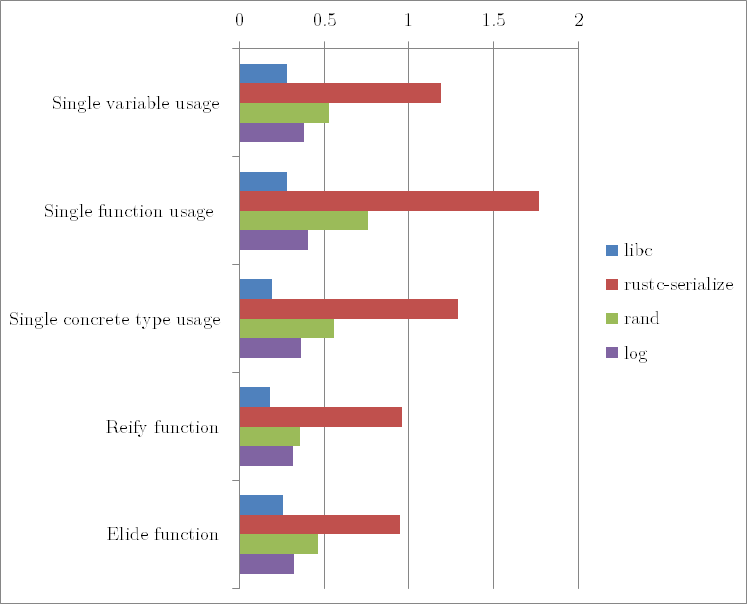
\includegraphics{refactorings}
}
\caption{Graph displaying results of the different refactorings}
\label{Fig:compareref}
\end{center}
\end{figure}

\subsection{Scalability of renames}
Since the renamings should follow the same general pattern inside the tool, exploring variation with a single type of renaming on a single crate should show the general relationship. In particular, `libc' was chosen for having a wider variety of occurrence counts specifically with concrete types. Other crates or types of renamings had few examples and only a limited amount of variation.

\begin{figure}[H]
\begin{center}
    \begin{tabular}{ | l | c |}
    \hline
    \textbf{Number of replaced occurrences} & \textbf{Time in seconds} \\ \hline
    1 type usage &  0.1925  \\ \hline
    3 type usages &  0.3821  \\ \hline
    4 type usages &   0.4749  \\ \hline
    6 type usages &   0.6737  \\ \hline
    8 type usages &   0.8739 \\ \hline
    13 type usages  &  1.373 \\ \hline
    29 type usages &  2.960  \\ \hline
    51 type usages &  5.059 \\ \hline
    \end{tabular}
\end{center}

\caption{Timings for varying usage counts of concrete types in libc}
\label{Fig:scaling}
\end{figure}

\begin{figure}[H]
\begin{center}
\scalebox{0.8}{
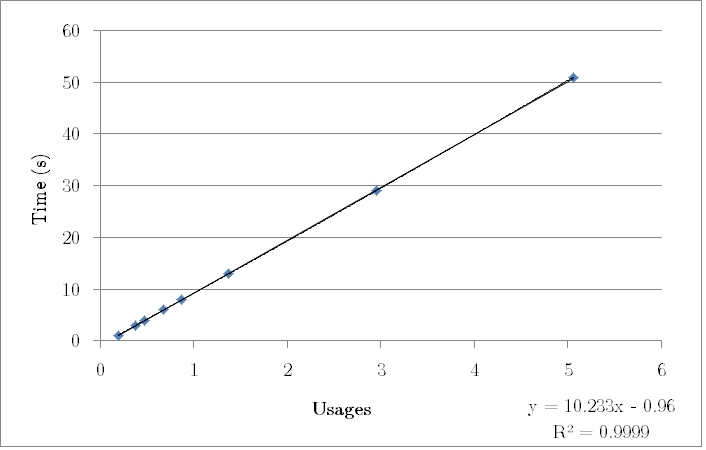
\includegraphics{scaling}
}
\caption{Graph displaying results of varying the number of usages}
\label{Fig:comparerefs}
\end{center}
\end{figure}


\begin{center}
\begin{fig}
\scalebox{0.9}{
\begin{tabular}{ l | l | l }
Rename &
Move &
Extract Method \\
Extract Local Variable &
Extract Constant &
Inline \\
Move Type to New File &
Extract Superclass &
Extract Interface \\
Push Down &
Pull Up &
Extract Class \\ 
Introduce Indirection &
Introduce Factory &
Introduce Parameter \\
Encapsulate Field &
Generalize Declared Type &
Migrate JAR File \\
Change Method Signature &
Convert Anon. Class to Nested &
Convert Local Variable to Field \\
Use Supertype Where Possible &
Introduce Parameter Object &
Infer Generic Type Arguments
\end{tabular}
}
\caption{List of refactorings supported by Eclipse}
\label{Fig:eclipse}
\end{fig}
\end{center}
